
\chapter{Information Theory and Rate Distortion Theory}
\label{ch01}


Please see below examples of equations using \verb+\begin{equation}+ \ldots
\verb+\end{equation}+ and \verb+align+.

The M\&C macros support various environments like:
constraint, construction, 
convention, conventions, corollary, definition, dictionary,
example, lemma, note, notation, observation, property, proposition,
remark, rules, theorem, etc.

What if you need an environment that the macros do not provide,
like ``guesswork?'' You create it with \verb+newMCtheorem+:

\verb+newMCtheorem}{guesswork}{GuessWork}+

\newMCtheorem{guesswork}{GuessWork}

\noindent
and use then use it:
\begin{guesswork}
This is pure guess work.
\end{guesswork}


\section{Introduction}
\label{ch01.sec1}

Thus far in the book, the term \textit{information}
\index{information}%
has been used sparingly and when
it has been used, we have purposely been imprecise as to its meaning.

\begin{figure}[hbt] % 01
\centering
  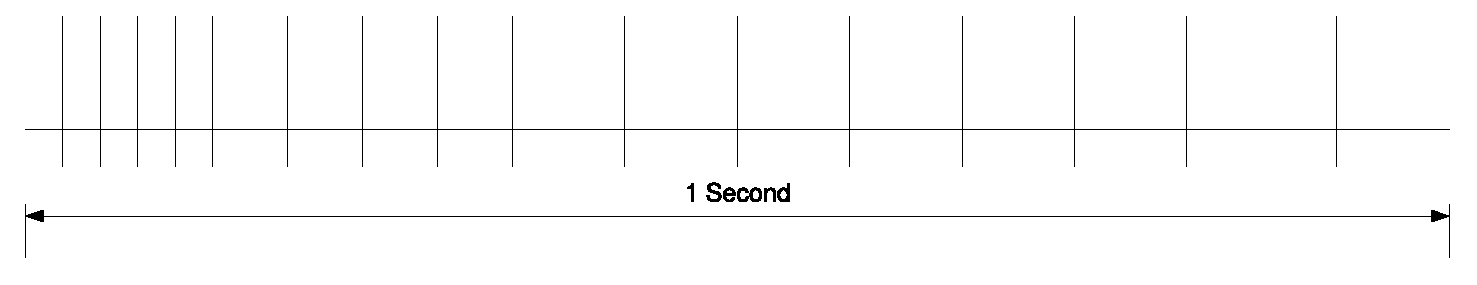
\includegraphics[width=3.3in]{line-spaces.eps}
\caption{Communication system block diagram.}
\label{ch01.fig1} 
\end{figure}

\begin{figure}[hbt] % 01
\centering
  \figboxes
\caption{Communication system block diagram.}
\label{ch01.fig2} 
\end{figure}

Examples of side-by-side figures.

%  F 2
\begin{figure}[hbt]%
\centering
\begin{subfigure}[t]{0.45\textwidth}%
	\smfigboxes
\caption{Annotated visualization of the structure of a biological neuron, reconstructed from electron microscope images of 30nm-thick slices of a mouse 
brain~\cite{tesniere59}.}%
\label{fig:bioneuron}%
\end{subfigure}%
\qquad%
\begin{subfigure}[t]{0.45\textwidth}%
	\smfigboxes
\caption{The shape of an action potential. A small external voltage stimulus (blue) triggers a cascade of charge build-up inside a neuron (red) via voltage-gated ion channels. The activation threshold is shown as a dotted line. Simulated using a Hodgkin-Huxley model of a neuron~\protect\cite{weber-97}.}%
\label{fig:ap}%
\end{subfigure}%
\caption{The structure and operation of biological neurons.}%
\end{figure}

%  F 3
\begin{figure}[b]
\centering
\begin{subfigure}[t]{0.45\textwidth}
	\smfigboxes
\caption{Points in $\mathbb{R}^2$, subdivided by a single linear classifier. One simple way of understanding linear classifiers is as a line (or hyper-plane, in higher dimensions) which splits space into two regions. In this example, points above the line are mapped to class 1 (red); those below, to class 0 (blue).}
\label{subfig:linclass}
\end{subfigure}%
\qquad%
\begin{subfigure}[t]{0.45\textwidth}
	\smfigboxes
\caption{Points in $\mathbb{R}^2$, subdivided by a combination of four linear classifiers. Each classifier maps \emph{all} points to class 0 or 1, and an additional linear classifier is used to combine the four. This hierarchical model is strictly more expressive than any linear classifier by itself.}
\label{subfig:circclass}
\end{subfigure}%
\caption{Simple elements can be combined to express more complex relationships.
This is one basic tenet of deep neural networks.}
\label{fig:classifiers}
\end{figure}


\section{Entropy and Average Mutual Information}
\label{ch01.sec2}

Consider a discrete random variable $U$ that takes on
the values $\{u_1, u_2, \dots, u_M\}$, where the set of possible
values of $U$ is often called the \textit{alphabet} and the elements
of the set are called \textit{letters} of the alphabet. Let $P_U(u)$
denote the probability  assignment  over the alphabet, then we can
define the \textit{self-information} of the event $ u = u_j $ by
\begin{equation}
  I_U \left( u_j \right) = \log \frac{1}{P_U (u_j)} = - \log P_U
    \left( u_j \right).
\label{ch01.eq1}
\end{equation}

\begin{example}
\label{ch01.ex1}
Given a random variable $U$ with four equally likely letters
in its alphabet, we wish to find $H(U)$. Clearly, $M=4$
and $P_U(u_i)= \tfrac{1}{4}$ for $ i = 1, 2, 3, 4 $.

\begin{align}
    I_{W;X}\left(w_j;x_k\right)
    & = \log
    \frac{P_{WX}\left(w_j, x_k\right)}{P_W\left(w_j\right)
              P_X\left(x_k\right)}
    \notag\\
    & = \log
    \frac{P_{X|W} \left( x_k | w_j\right)} {P_X \left(x_k\right)}
    =
     I_{X;W} \left(x_k; w_j\right).
\label{ch01.eq2}
\end{align}
\end{example}

\begin{property}
\label{ch01.pro1}
Let $U$ be a random variable with possible values $\{u_1,u_2,\dots, u_M\}$.
\end{property}

Example~\ref{ch01.ex1} illustrates Property~\ref{ch01.pro1}.

\begin{property}
\label{ch01.pro2}
Let $W$ and $X$ be jointly distributed random variables.
\end{property}

\begin{example}
\label{ch01.ex2}
Here we wish to calculate the mutual information and the average
mutual information for the probability assignments
(with $M=2$ and $N=2$)
\begin{equation}
 P_W \big(w_1\big) = P_W \big(w_2\big) = \tfrac{1}{2}
\label{ch01.eq3}
\end{equation}
\end{example}

\begin{example}[\cite{Boeringer}]
\label{ch01.ex3}
The source output is a ternary-valued random variable that takes on the
values $\{ u_1, u_2, u_3 \}$ with probabilities
$P(u_1) = 0.7, P(u_2) = 0.15 = P(u_3)$. 
\end{example}

\begin{theorem}[(Source Coding Theorem).]
\label{ch01.th1}
For a DMS with entropy $H(U)$,
the minimum average codeword length per source letter $(\bar{n})$ for any
code is lower
bounded by $H(U)$, that is, $\bar{n} \geq H(U)$, and further, $\bar{n}$
can be made as close to $H(U)$
as desired for some suitably chosen code.
\end{theorem}

\begin{theorem}[(Channel Coding Theorem~\cite{Wen-ChungLiu2005}).]
\label{ch01.th2}
Given a DMS
with entropy $H$ bits/source letter and a DMC with capacity $C$
bits/source letter,
if $H \leq C$, the source output can be encoded for transmission over
the channel with
an arbitrarily small bit error probability. Further, if $H > C$, the bit error
probability is bounded away from $0$.
\end{theorem}

\begin{proof}
This result can be proved in several ways, including calculus of
variations~\cite{WenWangetal2005} inequality; however, an
alternative method is used here.
\end{proof}

\begin{table}[hbt]
\caption{Timer0 Compare Output Mode, non-PWM Mode}
\label{ch01.tab1} 
\begin{center}
\begin{tabular}{|c|l|}
    \cb COM0x1-0
  & \cb Description 
\\
    \cw 00
  & \cw Normal port operation
\\
    \cy 01
  & \cy Toggle on Compare Match
\\
    \cw 10
  & \cw Clear on Compare Match
\\
    \cy 11
  & \cy Set on Compare Match
\\
\hline
\end{tabular}
\end{center}
\end{table}


\begin{center}
\begin{tabular}{|cl|}
    \cb COM0x1-0
  & \cb Description 
\\
    \cw 00
  & \cw Normal port operation
\\
    \cy 01
  & \cy Toggle on Compare Match
\\
    \cw 10
  & \cw Clear on Compare Match
\\
    \cy 11
  & \cy Set on Compare Match
\\
\hline
\end{tabular}
\end{center}


\section*{Summary}

In this chapter we have discussed very briefly some of the salient
results from information theory and rate distortion theory and have
indicated how these results can be used to bound communication system
performance.


\section*{Problems}
\index{problems}%

\begin{problems}

\item
A random variable $U$ has a sample space consisting of the set
of all possible binary sequences of length $N$, denoted
$\{u_j, j=1, 2, \ldots, 2^N \}$.

\item
Given a random variable $U$ with the alphabet $\{ u_1, u_2, u_3, u_4 \}$
and probability assignments $P(u_1) = 0.8, P(u_2)=0.1$,
$P(u_3) = 0.05, P(u_4)=0.05$, calculate the entropy of $U$.
Compare your result to a random variable with equally likely values.

\end{problems}

\clearpage

